\documentclass[10pt,a4paper]{article}
\usepackage[a4paper,margin=18mm,headheight=14pt]{geometry}
\usepackage[T1]{fontenc}
\usepackage{lmodern}
\usepackage{microtype}
\usepackage{xcolor}
\usepackage{graphicx}
\usepackage{booktabs}
\usepackage{tabularx}
\usepackage{array}
\usepackage{enumitem}
\usepackage{fancyhdr}
\usepackage{hyperref}
\usepackage{tikz}
\usetikzlibrary{arrows.meta,positioning,shapes.geometric,fit}

\definecolor{navy}{HTML}{10253F}
\definecolor{blue}{HTML}{1677FF}
\definecolor{cyan}{HTML}{18A7B5}
\definecolor{green}{HTML}{17835C}
\definecolor{amber}{HTML}{D88916}
\definecolor{red}{HTML}{C83D4D}
\definecolor{ink}{HTML}{263442}
\definecolor{muted}{HTML}{667483}
\definecolor{line}{HTML}{D7E0E8}
\definecolor{paper}{HTML}{F5F8FB}

\hypersetup{colorlinks=true,linkcolor=navy,urlcolor=blue,pdftitle={STRIVE: End-to-End Project Overview},pdfauthor={Team Null Pointer},pdfsubject={Technical and product overview of STRIVE 0.2.0}}
\setlength{\parindent}{0pt}
\setlength{\parskip}{5pt}
\setlist[itemize]{leftmargin=5mm,itemsep=2pt,topsep=3pt}
\setlist[enumerate]{leftmargin=6mm,itemsep=3pt,topsep=3pt}
\renewcommand{\arraystretch}{1.25}
\pagestyle{fancy}
\fancyhf{}
\lhead{\small\textcolor{muted}{STRIVE \textbullet\ Project Overview}}
\rhead{\small\textcolor{muted}{Repository snapshot: 15 Sep 2026}}
\cfoot{\small\textcolor{muted}{\thepage}}
\newcommand{\sectionrule}{\vspace{-2mm}\textcolor{blue}{\rule{22mm}{1.2pt}}\vspace{2mm}}
\newcommand{\callout}[2]{\vspace{2mm}\noindent\fcolorbox{#1}{paper}{\parbox{0.94\linewidth}{\textbf{\textcolor{#1}{#2}}}}\vspace{2mm}}
\newcommand{\code}[1]{\texttt{\small #1}}
\newcolumntype{Y}{>{\raggedright\arraybackslash}X}
\newcolumntype{L}[1]{>{\raggedright\arraybackslash}p{#1}}

\begin{document}

\begin{titlepage}
\pagecolor{navy}
\color{white}
\vspace*{20mm}
{\Huge\bfseries STRIVE\par}
\vspace{3mm}
{\Large Streaming Training-free Real-time\\Identity-Verification Engine\par}
\vspace{12mm}
\textcolor{cyan}{\rule{45mm}{2pt}}
\vspace{12mm}
{\LARGE\bfseries End-to-End Project Overview\par}
\vspace{6mm}
{\large What the project does, how it works, how to run it,\\and what remains before real-world deployment\par}
\vfill
\begin{tabular}{@{}ll}
Project & AI-powered real-time voice-cloning risk and prevention prototype\\
Context & Smart India Hackathon 2026 \textbullet\ SIH26104\\
Team & Null Pointer\\
Version & 0.2.0\\
Snapshot & Repository commit \texttt{2821d16}, with local in-progress changes\\
Prepared & 15 September 2026\\
\end{tabular}
\vspace{16mm}

{\small\textcolor{line}{This document distinguishes implemented mechanics, recorded fixture evidence, and unvalidated research claims.}}
\end{titlepage}
\nopagecolor
\color{ink}

\tableofcontents
\newpage

\section{The project in one page}
\sectionrule

STRIVE is a prototype for reducing fraud during voice calls where an attacker may use a cloned or substituted voice. It continuously analyzes a call, presents several kinds of acoustic evidence, combines that evidence with the business context of the requested action, and can hold a sensitive action until the caller is verified through a channel outside the voice call.

Its key product idea is that detection is not the final step. A risk score becomes useful only when it drives a safe workflow: continue monitoring, request verification, hold the action, release it after successful verification, or block and escalate after failure.

\callout{blue}{Core principle: authenticity risk, business-context risk, and the final decision risk are deliberately separate. A noisy channel is weak evidence, not proof of a fake voice. A low acoustic score is not identity verification.}

\begin{tabularx}{\linewidth}{@{}L{36mm}Y@{}}
\toprule
\textbf{Question} & \textbf{Answer}\\
\midrule
Who is it for? & Banks, contact centers, support desks, and other workflows where a caller asks for a sensitive action.\\
What enters? & Browser microphone PCM, uploaded call audio, or a deterministic presentation scenario.\\
What comes out? & Per-window evidence, authenticity state, context risk, decision risk, explanations, latency, channel quality, and a recommended action.\\
What is implemented? & Streaming mechanics, API, dashboard, procedural demo mode, session-profile logic, policy workflow, audit metadata, research adapters, evaluation tools, and an optional Rust audio runtime.\\
What is not proven? & Real-world voice-clone detection accuracy, calibrated probabilities, Indic-language fairness, unseen-generator robustness, production scale, or real banking/callback integration.\\
\bottomrule
\end{tabularx}

The default experience is intentionally labeled \textbf{DEMO DSP}. It uses procedural signals and a small synthetic reference index to prove that the end-to-end software and prevention workflow operate. It must not be presented as a neural deepfake detector benchmark.

\section{The problem STRIVE addresses}
\sectionrule

Voice cloning makes caller identity harder to judge by ear. A conventional call flow may authenticate the user once and then allow a high-value action based on what is said during the call. STRIVE instead treats the call as a changing stream and continuously asks three questions:

\begin{enumerate}
\item Does the current audio resemble known genuine or spoof-like reference examples?
\item Is the current voice consistent with the cautiously established voice profile from earlier in this same call?
\item Is the transition around the newest audio boundary locally coherent?
\end{enumerate}

These questions are supporting evidence, not identity proof. STRIVE then asks a fourth, non-acoustic question: how risky is the requested business action? A large urgent transfer to a new beneficiary should receive stricter treatment than a routine low-risk request, even if the acoustic evidence is inconclusive.

\subsection{Project goals}

\begin{itemize}
\item Analyze audio incrementally rather than waiting for a full recording.
\item Expose uncertainty, missing evidence, freshness, channel reliability, and reasons.
\item Build a temporary in-call profile without requiring prior voice enrollment.
\item Keep audio-risk scoring separate from policy and transaction context.
\item Demonstrate a safe hold-and-verify response that does not rely on the suspect voice channel.
\item Preserve privacy by keeping raw audio and embeddings transient by default.
\item Provide a reproducible path from engineering fixtures to frozen research models and held-out evaluation.
\end{itemize}

\subsection{Explicit non-goals of the current MVP}

The repository does not implement SIP/RTP interception, Asterisk, Teams/Zoom integration, real money movement, real MFA/callback providers, production IAM, horizontally distributed state, or a legally certified biometric system. It also does not ship pretrained model weights or a speech corpus.

\section{End-to-end user journey}
\sectionrule

\begin{enumerate}
\item \textbf{Start a call session.} The client creates an ephemeral call with an optional language hint and business context such as amount, urgency, new beneficiary, or privileged request.
\item \textbf{Stream audio.} A browser microphone, uploaded recording, or scenario supplies audio. The canonical detector contract is 16 kHz, mono PCM.
\item \textbf{Warm up and establish evidence.} The system waits for enough active speech. During the first five seconds it decides whether the early audio is trustworthy enough to seed a temporary same-call profile.
\item \textbf{Score overlapping windows.} Two-second windows are produced at a configurable hop. Presentation and live presets use a 0.5-second hop. The engine measures activity, channel condition, reference evidence, session consistency, and boundary coherence.
\item \textbf{Fuse and explain.} Available tracks are reliability-masked, weights are renormalized, and an exponential moving average smooths the authenticity risk. Missing evidence remains unavailable; it is never silently converted to zero.
\item \textbf{Apply business policy.} The policy combines authenticity risk with context risk to recommend continued monitoring, verification, holding, or escalation.
\item \textbf{Resolve the action.} A simulated registered-number callback, MFA check, or supervisor review records an outcome. Verified can release the current action; failure blocks and escalates; review stays held.
\item \textbf{End and erase.} Closing or expiring a call clears its ring buffer, temporary profile, queued windows, and upload memory. The audit retains only allow-listed metadata.
\end{enumerate}

\begin{center}
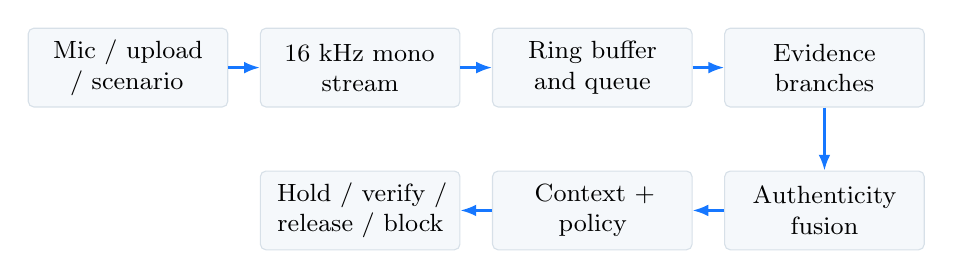
\begin{tikzpicture}[node distance=5mm and 4mm, every node/.style={font=\small}, box/.style={draw=line,rounded corners=2pt,fill=paper,minimum height=10mm,text width=23mm,align=center}, arr/.style={-{Latex[length=2mm]},thick,draw=blue}]
\node[box] (input) {Mic / upload / scenario};
\node[box,right=of input] (norm) {16 kHz mono\\stream};
\node[box,right=of norm] (window) {Ring buffer\\and queue};
\node[box,right=of window] (evidence) {Evidence\\branches};
\node[box,below=8mm of evidence] (fusion) {Authenticity\\fusion};
\node[box,left=of fusion] (policy) {Context +\\policy};
\node[box,left=of policy] (action) {Hold / verify /\\release / block};
\draw[arr] (input)--(norm); \draw[arr] (norm)--(window); \draw[arr] (window)--(evidence);
\draw[arr] (evidence)--(fusion); \draw[arr] (fusion)--(policy); \draw[arr] (policy)--(action);
\end{tikzpicture}
\end{center}

\section{System architecture}
\sectionrule

\subsection{Input and capture layer}

\textbf{Python service.} FastAPI serves the dashboard and exposes REST and WebSocket endpoints. The presentation path currently supports text WebSocket messages containing Base64 signed 16-bit PCM, plus streamed upload/scenario playback. Audio decode supports WAV/FLAC and FFmpeg-backed compressed formats, with 20 MiB and 120-second presentation limits.

\textbf{Live binary design.} The repository also contains a \code{pcm-v2} design: 20 ms binary packets, independent receiver and scorer tasks, and a one-window freshest-first queue. The optional Rust runtime implements this design with isolated persistent Python detector workers. In the current local working tree, the Python API launcher still exposes the legacy text WebSocket handler; see Section~\ref{sec:status}.

The ring buffer makes overlapping windows. Capture and inference are separated inside the engine. When the bounded queue overflows, the oldest pending window is discarded so the latest state remains useful. The loss is counted, continuity is reset, and the next event reports \code{CAPTURE\_QUEUE\_OVERFLOW}.

\subsection{Evidence layer}

\begin{tabularx}{\linewidth}{@{}L{35mm}L{38mm}Y@{}}
\toprule
\textbf{Track} & \textbf{Implemented meaning} & \textbf{Important limitation}\\
\midrule
Artifact / global & k-nearest-neighbor ratio over a labeled reference index in the countermeasure embedding space. & Demo labels are procedural families, not genuine/spoof speech. Research quality depends on models and a licensed, disjoint corpus.\\
Session consistency & Distance from a trust-gated temporary profile built only from accepted windows in this call. & Detects within-call change, not the caller's real-world identity; can be attacked during bootstrap or by slow drift.\\
Boundary coherence & Distance between adjacent segment representations around the new-audio seam. & Weak supporting cue; phonetic change, gaps, and packet loss may confound it.\\
Channel quality & Bandwidth estimate, SNR proxy, clipping, level, discontinuity, and optional transport metadata. & Reliability only. Poor telephony quality is not spoof evidence.\\
\bottomrule
\end{tabularx}

The session profile uses separate FAISS indexes for profile vectors and phoneme/segment vectors. It accepts at most 120 windows per call and is cleared on teardown or gap. A gap also blocks reuse of trust established before the interruption.

\subsection{Fusion and decision logic}

For available acoustic scores $s_i$, scheduled weights $w_i$, and reliability $r_i$, STRIVE computes a normalized raw fusion:
\[
R_{raw}=\frac{\sum_i w_i r_i s_i}{\sum_i w_i r_i}, \qquad
R_t=\alpha R_{t-1}+(1-\alpha)R_{raw}, \quad \alpha=0.70.
\]

Unavailable tracks receive zero weight and active weights are renormalized. Global evidence is mandatory for a public acoustic result. A common channel reliability factor cannot change a valid normalized score because it cancels across tracks; sufficiently unusable audio can make the engine abstain.

\begin{tabular}{@{}lccc@{}}
\toprule
\textbf{Audio age} & \textbf{Global} & \textbf{Session} & \textbf{Coherence}\\
\midrule
Under 15 s & 0.80 & 0.00 & 0.20\\
15--60 s & 0.50 & 0.30 & 0.20\\
Over 60 s & 0.30 & 0.50 & 0.20\\
\bottomrule
\end{tabular}

Acoustic thresholds are 0.50 for review, 0.75 for high, and 0.90 for critical. These values are engineering settings, not calibrated probabilities.

Context risk is rule-based: amount bands contribute up to 0.35, urgency 0.20, a new beneficiary 0.25, and a privileged request 0.20. The policy computes
\[
R_{decision}=1-(1-R_{auth})(1-0.5R_{context}).
\]
If authenticity is unavailable and context is high, the system fails safely by recommending hold and verify.

\section{Prevention workflow}
\sectionrule

The project treats risk as an input to a state machine rather than a verdict printed on a dashboard.

\begin{center}
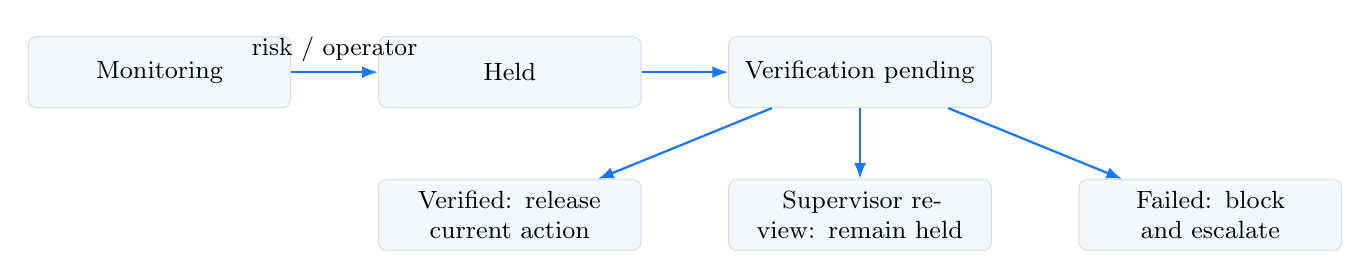
\begin{tikzpicture}[node distance=9mm and 11mm, every node/.style={font=\small}, state/.style={draw=line,rounded corners=3pt,fill=paper,minimum height=9mm,text width=31mm,align=center}, arr/.style={-{Latex[length=2mm]},thick,draw=blue}]
\node[state] (monitor) {Monitoring};
\node[state,right=of monitor] (held) {Held};
\node[state,right=of held] (pending) {Verification pending};
\node[state,below left=of pending] (release) {Verified: release current action};
\node[state,below=of pending] (review) {Supervisor review: remain held};
\node[state,below right=of pending] (block) {Failed: block and escalate};
\draw[arr] (monitor)-- node[above]{risk / operator} (held);
\draw[arr] (held)--(pending);
\draw[arr] (pending)--(release); \draw[arr] (pending)--(review); \draw[arr] (pending)--(block);
\end{tikzpicture}
\end{center}

The hold is latched: a later drop in acoustic risk does not automatically undo it. Verification is scoped to the current evidence epoch so an old success cannot authorize a later changed call. All verification buttons are simulations and do not contact external providers.

\section{Software map}
\sectionrule

\begin{tabularx}{\linewidth}{@{}L{42mm}Y@{}}
\toprule
\textbf{Area} & \textbf{Responsibility}\\
\midrule
\path{strive/audio.py} & Decode, normalize, activity gating, window and ring-buffer mechanics.\\
\path{strive/capture.py} & Bounded pending-window queue and capture/drop telemetry.\\
\path{strive/engine.py} & Per-call lifecycle, bootstrap, parallel evidence jobs, fusion, explanations, and event schema.\\
\path{strive/features.py} & DSP surrogate and acoustic profile features.\\
\path{strive/retrieval.py} & Labeled global FAISS index and temporary session-profile indexes.\\
\path{strive/channel.py} & Channel measurements and reliability scalar.\\
\path{strive/policy.py} & Business context score and action recommendation.\\
\path{strive/api.py} & FastAPI lifecycle, REST/WebSocket routes, authentication, uploads, workflow, metrics, and static UI.\\
\path{strive/audit.py} & SQLite metadata audit with an explicit allow-list.\\
\path{strive/models/research.py} & Fail-closed adapters for sealed local frozen models.\\
\path{strive/streaming.py} & Binary full-duplex Python transport design.\\
\path{native/audio-runtime/} & Optional Rust packet ingestion, fixed-allocation buffering, worker supervision, and process isolation.\\
\path{web/} & Browser dashboard, scenario/upload controls, microphone capture, and AudioWorklet.\\
\path{scripts/} & Launchers, preflight, model preparation, indexing, evaluation, benchmarks, evidence, and release packaging.\\
\path{tests/} and \path{evidence/} & Automated contracts and recorded benchmark receipts.\\
\bottomrule
\end{tabularx}

\section{Operating modes and interfaces}
\sectionrule

\subsection{Demo DSP mode}

Default mode. It uses \code{dsp-surrogate-v1} and a 48-vector procedural index. Three presentation scenarios are available: stable/genuine-like, suspicious from the start, and mid-call source replacement at 15 seconds. They are deterministic workflow fixtures, not human recordings or neural accuracy tests.

\subsection{Research mode}

Research mode loads only locally prepared and sealed assets. It refuses missing files, checksum mismatches, wrong input geometry, fixture indexes, incompatible model/index identifiers, and invalid dimensions. It does not silently fall back to demo scoring.

The planned stack uses a frozen NII anti-deepfake countermeasure encoder, an XLSR phoneme model, optional SpeechBrain language identification, a labeled FAISS reference index, and either the documented 62-dimensional acoustic profile or explicit externally exported Vox trait modules. Weights and corpora are intentionally absent from the repository.

\subsection{Offline replay}

\path{STRIVE_Demo.html} is a portable fallback that replays captured API events. It has no model, live microphone, upload analysis, or new inference.

\subsection{External interface}

The service exposes health, readiness, configuration, status, metrics, call creation/state/deletion, audio chunks, upload, context updates, hold, verification, transaction simulation, audit, batch analysis, scenarios, and a primary stream WebSocket. OpenAPI is available at \path{/docs}. Non-loopback binding requires an API token.

\section{Privacy, safety, and security design}
\sectionrule

\begin{itemize}
\item Raw uploaded audio, live PCM, temporary embeddings, and session profiles are not written to the audit store by default.
\item Upload buffers are held in memory and overwritten on playback completion, replacement, or teardown. This is lifecycle cleanup, not a forensic secure-erasure guarantee.
\item Audit entries retain allow-listed metadata such as risks, track scores, reasons, actions, mode, model version, workflow, and latency.
\item Requests have size limits; calls have duration, idle, and concurrency limits; out-of-order frames are rejected.
\item Loopback access can operate without a token. Binding beyond loopback requires \code{STRIVE\_API\_TOKEN}; HTTP uses bearer authentication and WebSocket authentication occurs in the first message.
\item Same-origin checks, a restrictive Content Security Policy, no-store caching, and basic security headers are applied.
\item Model loading is offline at runtime. Research assets are hashed and compatibility-checked.
\end{itemize}

Voice embeddings may be biometric or personal data. The repository's transient handling reduces exposure, but production use still requires consent, retention rules, access controls, encryption, legal review, and a formal threat model.

\section{How to run the project}
\sectionrule

\subsection{Fast presentation path}

Linux/macOS/WSL:
\begin{verbatim}
./scripts/presentation.sh
\end{verbatim}

Windows PowerShell:
\begin{verbatim}
.\scripts\presentation.ps1
\end{verbatim}

The launcher performs preflight checks, starts a loopback server, and opens or prints \path{http://127.0.0.1:8000}. The recommended demo is \emph{Mid-Call Voice Replacement}, followed by \emph{Hold \& Verify} and a failed or verified simulated outcome.

\subsection{Manual demo setup}

\begin{verbatim}
python3.12 -m venv .venv
.venv/bin/python -m pip install -r requirements-demo.lock
.venv/bin/python -E scripts/start.py
\end{verbatim}

FFmpeg is optional for WAV/FLAC and required for compressed upload formats. On this development machine, \code{-E} avoids a host-level Python package injector that can shadow virtual-environment dependencies.

\subsection{Docker}

\begin{verbatim}
export STRIVE_API_TOKEN='choose-a-long-secret'
docker compose up --build
\end{verbatim}

Compose binds port 8000 to loopback, stores the metadata audit in a volume, uses a 64 MiB temporary filesystem, and runs the container as a non-root user.

\subsection{Optional native runtime}

\begin{verbatim}
cargo build --release --locked \
  --manifest-path native/audio-runtime/Cargo.toml
.venv/bin/python -E scripts/start_native.py --port 8000
\end{verbatim}

Rust owns live packet validation, buffering, timestamps, bounded pending work, and worker recovery. Python retains detection, fusion, policy, and audit. Each admitted call receives a separate Python worker/model instance, so RAM/VRAM limits must be considered before increasing concurrency.

\section{Verification and measured evidence}
\sectionrule

Recorded repository evidence demonstrates software mechanics on a 12th-generation Intel i5 CPU using the DSP surrogate. A prior 2-second-window/0.5-second-hop multi-rate benchmark reported 22.92 ms p95 end-to-end compute/queue time and a 54.4x real-time factor. A paced loopback \code{pcm-v2} run reported 82.53 ms p95 completed-window-to-client latency, 400/400 acknowledged packets, and zero dropped windows. Browser evidence records a passing synthetic-microphone AudioWorklet flow.

These figures exclude physical microphone latency, WAN transport, neural inference, large research indexes, and browser rendering where noted. They are runtime measurements, not detection-quality metrics.

\begin{tabularx}{\linewidth}{@{}L{44mm}Y@{}}
\toprule
\textbf{Evidence that exists} & \textbf{Evidence still required}\\
\midrule
Windowing, overlap, sequence validation, masking, bootstrap, profile cleanup, API/workflow contracts, privacy allow-list, scheduler, overload handling, codec augmentation, and browser sample-rate conversion. & Genuine/spoof ROC-AUC, PR-AUC, EER, operating-point false positives/negatives, calibration, Indic-language/code-mix slices, unseen-generator tests, codec robustness on speech, attack-onset delay, and neural hardware latency.\\
\bottomrule
\end{tabularx}

\subsection{Fresh snapshot check}\label{sec:status}

This PDF was generated from commit \code{2821d16} with an already modified/untracked working tree. The fresh checks performed for this document found:

\begin{itemize}
\item Dashboard and AudioWorklet JavaScript syntax passed.
\item AudioWorklet framing passed for 16 kHz, 44.1 kHz, and 48 kHz inputs.
\item The Python suite reached 90 passing tests before the first failure.
\item The first failure is an integration mismatch: \path{tests/test_live_stream.py} expects a \code{pcm-v2} WebSocket handshake field, while the current \path{strive/api.py} stream path returns the older ready message and text/Base64 protocol. The binary transport implementation exists in \path{strive/streaming.py} and in the Rust runtime, but it is not wired into the current Python API route in this snapshot.
\end{itemize}

Therefore, older repository notes claiming a completely passing expanded suite should be treated as historical receipts, not the status of this locally modified snapshot.

\section{Known limitations and technical risks}
\sectionrule

\begin{enumerate}
\item \textbf{Accuracy is unvalidated.} Demo scores show software behavior only. No real speech corpus or neural-model results ship with the project.
\item \textbf{Risk is uncalibrated.} A score of 0.8 is not an 80\% probability of fraud.
\item \textbf{Fusion can dilute strong global evidence.} After 60 seconds, a global score of 1.0 with stable session/coherence tracks can fuse to 0.30 before smoothing.
\item \textbf{EMA delays escalation.} From zero, three maximum raw updates produce 0.657; five produce about 0.832. This can delay an alert.
\item \textbf{Bootstrap is not identity proof.} The early voice may already be fraudulent, and gradual profile poisoning remains an open threat.
\item \textbf{Continuity is a weak cue.} Natural phonetic transitions, packet loss, and channel changes can resemble discontinuities.
\item \textbf{Channel metrics are incomplete.} Waveform analysis did not detect the tested short packet erasures; packet-loss rate must be supplied by the transport.
\item \textbf{Production integration is absent.} There is no SIP adapter, external identity provider, banking system, full monitoring stack, or production authorization layer.
\item \textbf{Scaling is bounded.} The Python default is a single process with up to eight sessions. The native path isolates workers but duplicates model memory per call.
\end{enumerate}

\section{From prototype to validated system}
\sectionrule

The repository already contains the preparation and evaluation scaffolding. Completing the project responsibly means executing the following sequence with real assets and preserving negative results:

\begin{enumerate}
\item \textbf{Obtain approved assets.} Review model licenses, obtain consented genuine speech and legally generated spoof speech, and document provenance.
\item \textbf{Prepare frozen models.} Download pinned upstream revisions in an explicit online step, export the NII model in its compatible environment, compare eager and exported outputs, then hash and seal the bundle.
\item \textbf{Build a disjoint reference index.} Use both genuine and spoof examples. Keep source IDs, speakers, and augmentations from leaking between reference, validation, and test splits.
\item \textbf{Run research mode fail-closed.} Verify geometry, dimensions, model/index fingerprint, checksums, and local-only loading.
\item \textbf{Evaluate all evidence combinations.} Compare each single track, every pair, and the full ensemble on a common eligible cohort. Report abstentions as well as scores.
\item \textbf{Test operational conditions.} Slice results by language, code-mix, speaker, generator, codec, noise, packet loss, and attack onset. Measure false-positive cost and time to hold.
\item \textbf{Calibrate and revise policy.} Select operating points from validation data, then lock them before final testing. Revisit the age schedule, global-evidence floor, and bootstrap defenses.
\item \textbf{Integrate and harden.} Add telephony adapters, real out-of-band verification, authorization, encrypted storage, monitoring, process isolation, capacity tests, incident response, and human review procedures.
\item \textbf{Pilot safely.} Run in shadow mode first, measure subgroup harms and operational overrides, and require human approval before enforcing sensitive decisions.
\end{enumerate}

\callout{green}{The strongest current contribution is the end-to-end architecture and its honest uncertainty handling: streaming evidence is connected to a privacy-aware, fail-safe prevention workflow. The central remaining question is empirical---whether the research stack detects real attacks accurately and fairly enough to justify deployment.}

\section{Suggested demonstration narrative}
\sectionrule

\begin{enumerate}
\item Explain that STRIVE monitors a call continuously and does not claim identity from one low score.
\item Keep a high-risk context visible, such as INR 10,00,000, urgent, and a new beneficiary. Point out that acoustic and business risks remain separate.
\item Run the deterministic mid-call replacement scenario in real-time presentation mode.
\item During warm-up, show the analyzing state and explain the trust-gated temporary profile.
\item At the source-change marker, show the artifact, session, continuity, channel, freshness, and reason fields.
\item When policy requests review or a hold, click \emph{Hold \& Verify}. Emphasize that the sensitive action is paused while the conversation may continue.
\item Select callback, MFA, or supervisor review. Show both the verified-release path and the failed-block/escalate path.
\item Close with the engineering status panel and state clearly that fixture scores and DSP latency are not neural accuracy evidence.
\end{enumerate}

\section{Glossary and source map}
\sectionrule

\begin{tabularx}{\linewidth}{@{}L{34mm}Y@{}}
\toprule
\textbf{Term} & \textbf{Meaning in STRIVE}\\
\midrule
CM & Countermeasure representation used for global reference retrieval.\\
SPS & Same-call speaker/session profile store; temporary and trust-gated.\\
Authenticity risk & Acoustic anomaly score from available evidence tracks.\\
Context risk & Rule-based risk of the requested business action.\\
Decision risk & Policy combination of authenticity and context risk.\\
Abstention & No acoustic score because evidence is missing, stale, silent, unreliable, or failed.\\
Fixture & Deterministic synthetic signal used to exercise software, not to measure detection accuracy.\\
\bottomrule
\end{tabularx}

Primary repository sources used for this overview: \path{README.md}; \path{docs/ARCHITECTURE.md}; \path{docs/API.md}; \path{docs/MODELS.md}; \path{docs/REQUIREMENTS.md}; \path{docs/VALIDATION.md}; \path{docs/LATENCY.md}; \path{docs/NATIVE_AUDIO.md}; \path{docs/CODEC_BENCHMARK.md}; runtime code under \path{strive/}; launch and evaluation utilities under \path{scripts/}; the browser client under \path{web/}; tests under \path{tests/}; and recorded receipts under \path{evidence/}.

\vfill
\begin{center}
\textcolor{muted}{\small End of overview \textbullet\ STRIVE 0.2.0 \textbullet\ Team Null Pointer}
\end{center}

\end{document}
